\section{Introduction}

L’analyse des besoins représente une étape clé dans le processus de développement d’une solution informatique. Elle vise à comprendre le contexte du projet, à identifier les différents acteurs impliqués et à préciser les attentes auxquelles le système devra répondre. Une analyse rigoureuse permet ainsi de poser des bases solides pour les phases ultérieures, en assurant une meilleure adéquation entre la solution proposée et les besoins réels.

Dans le cadre de ce travail, cette étape s’inscrit dans une démarche globale de développement structurée, dont les différentes phases seront brièvement présentées à travers la section consacrée à la méthodologie suivie. Cette dernière permet de situer l’analyse des besoins dans l’enchaînement logique des étapes menant à la conception, à la réalisation et à la validation de la solution.

Ce chapitre est consacré à l’analyse des besoins de la solution RevMine. Il débute par la présentation de la méthodologie adoptée, puis s’intéresse à l’identification des acteurs du système ainsi qu’à la définition des besoins fonctionnels et non fonctionnels. Ces besoins sont ensuite validés afin de garantir leur cohérence et leur adéquation avec les objectifs du projet, avant d’être modélisés à travers des cas d’utilisation et des diagrammes d’activité. L’ensemble de cette analyse constitue une base essentielle pour la phase de conception qui sera abordée dans le chapitre suivant.

\section{Méthodologie Suivie}

Dans le cadre du développement de la solution RevMine, nous avons adopté une démarche méthodologique structurée et itérative, visant à assurer la qualité et la cohérence du système tout au long de son élaboration. Cette approche repose sur une progression par étapes successives, permettant d’affiner progressivement la solution en fonction des besoins identifiés.

La démarche suivie s’articule autour de quatre phases principales :

\textbf{Analyse des besoins.} Cette phase consiste à identifier et formaliser les exigences fonctionnelles et non fonctionnelles du système, à partir de l’étude des acteurs et des cas d’utilisation.

\textbf{Conception.} Elle vise à définir l’architecture globale de la solution en structurant le système en composants modulaires, tout en respectant des principes tels que la séparation des responsabilités et la maintenabilité.

\textbf{Réalisation.} L’implémentation est effectuée de manière itérative, à travers des cycles courts permettant l’intégration progressive des différents composants du système, avec un suivi continu de leur cohérence.

\textbf{Validation.} Cette phase repose sur la vérification des fonctionnalités développées à travers des tests d’intégration, afin de s’assurer de leur conformité avec les besoins définis.

Cette démarche permet ainsi de garantir une évolution maîtrisée de la solution, en assurant un alignement continu entre les besoins exprimés et le système réalisé.

\section{Etude des besoins}
\subsection{Identification des acteurs}
Les principaux acteurs identifiés interagissant avec le système RevMine sont les suivants :

\subsubsection*{Chercheur en ingénierie logicielle}

\textbf{Profil :} Doctorant, post-doctorant ou enseignant-chercheur menant des études empiriques sur les processus de développement logiciel.

\textbf{Besoins :}
\begin{itemize}
    \item Collecter des datasets sur plusieurs projets open source
    \item Réaliser des analyses statistiques sur les données de revue
    \item Reproduire et valider des études existantes
    \item Exporter les données pour des traitements externes (R, Python)
\end{itemize}

\subsubsection*{Praticien DevOps}

\textbf{Profil :} Développeur, lead technique ou DevOps engineer souhaitant optimiser les processus de son équipe.

\textbf{Besoins :}
\begin{itemize}
    \item Identifier les goulots d'étranglement dans le processus de revue
    \item Mesurer les temps de revue et détecter les anomalies
    \item Comparer les performances entre équipes ou projets
    \item Obtenir des indicateurs d'amélioration
\end{itemize}

\subsubsection*{Manager de projet}

\textbf{Profil :} Chef de projet, scrum master ou product owner responsable de la livraison.

\textbf{Besoins :}
\begin{itemize}
    \item Suivre les métriques de productivité de l'équipe
    \item Visualiser les tendances et l'évolution des pratiques
    \item Identifier les membres surchargés ou sous-utilisés
    \item Générer des rapports pour la direction
\end{itemize} 
\vspace{1em}
\vspace{1em}
En plus des acteurs humains, le système RevMine interagit avec des systèmes externes qui jouent un rôle essentiel dans son fonctionnement.

\subsubsection*{GitHub / GitLab}
\textbf{Profil :} Plateformes de gestion de code source fournissant les données de revue de code via leurs API.
\textbf{Rôle :}
\begin{itemize}
    \item Fournir les données relatives aux pull requests et merge requests
    \item Permettre l’accès aux commits, commentaires et métadonnées associées
    \item Gérer l’authentification et les permissions d’accès
\end{itemize}

\subsubsection*{Service LLM}
\textbf{Profil :} Service de traitement du langage naturel, pouvant être implémenté localement ou via un fournisseur externe.
\textbf{Rôle :}
\begin{itemize}
    \item Interpréter les requêtes utilisateur exprimées en langage naturel
    \item Générer des plans de collecte ou d’analyse
    \item Assister l’utilisateur dans l’exploration et l’analyse des données
\end{itemize}

\subsection{Besoins fonctionnels}

À partir des acteurs identifiés, il est possible de dériver les besoins du système RevMine. En effet, chaque catégorie d’utilisateur exprime des attentes spécifiques en termes de fonctionnalités et de contraintes d’utilisation. L’analyse de ces attentes permet de formaliser un ensemble de besoins fonctionnels, décrivant les services que le système doit fournir, ainsi que des besoins non fonctionnels, définissant les exigences de qualité et les contraintes auxquelles la solution doit satisfaire. Les sections suivantes présentent ces besoins de manière structurée.

\renewcommand{\arraystretch}{1.5}

\begin{center}
\begin{longtable}{|c|p{15cm}|}
    \caption{Spécifications fonctionnelles du système RevMine.}
    \label{tab:functional-specs} \\
    \hline
    \textbf{ID} & \textbf{Description} \\
    \hline
    \endfirsthead

    \hline
    \textbf{ID} & \textbf{Description} \\
    \hline
    \endhead

    \hline
    \multicolumn{2}{|r|}{\textit{Suite à la page suivante}} \\
    \hline
    \endfoot

    \hline
    \endlastfoot

    1 & Le système doit permettre la gestion des espaces de travail et des projets à analyser. \\\hline
    2 & Le système doit permettre la configuration des connexions GitHub et GitLab. \\\hline
    3 & Le système doit permettre la gestion d'authentification sécurisée (tokens API). \\\hline
    4 & Le système doit vérifier automatiquement les permissions, la disponibilité des end-points et la validité du token. \\\hline
    5 & Le système doit permettre la sélection des dépôts à analyser. \\\hline
    6 & Le système doit permettre la configuration des endpoints et l'application des filtres de manière manuelle. \\\hline
    7 & Le système doit générer un plan de collecte à partir d'un prompt en langage naturel. \\\hline
    8 & La plateforme doit permettre à l'utilisateur de valider, modifier ou affiner le plan de collecte généré avant exécution. \\\hline
    9 & Le système doit extraire les données de revue de code via les API des plateformes (Pull/Merge Requests, Commentaires, Commits, Reviewers et auteurs). \\\hline
    10 & Assurer une gestion robuste des appels API afin de prévenir les erreurs et pertes de données \\\hline
    11 & Le système doit permettre de stocker les données dans un format structuré. \\\hline
    12 & Le système doit offrir des fonctionnalités de nettoyage des données avant analyse. \\\hline
    13 & Le système doit permettre l’importation d’un dataset existant. \\\hline
    14 & Le système doit calculer automatiquement des métriques avancées telles que le délai de traitement, le taux de modification du code, l’entropie historique et l’engagement des relecteurs. \\\hline
    15 & Le système doit permettre à l'utilisateur de demander des analyses personnalisées en langage naturel. \\\hline
    16 & La plateforme doit permettre à l'utilisateur de sélectionner des analyses prédéfinies. \\\hline
    17 & Le système doit afficher les résultats d’analyse dans un tableau de bord interactif. \\\hline
    18 & Le système doit générer des résumés statistiques basés sur les métriques collectées. \\\hline
    19 & Le système doit permettre la génération de visualisations interactives prêtes à être exploitées pour l’analyse ou la publication. \\\hline
    20 & Le système doit permettre d'exporter les résultats. \\\hline
    21 & L’utilisateur doit être notifié de l’état d’avancement des opérations importantes. \\\hline
    22 & Le système doit permettre la collecte des données Kanban. \\\hline
    23 & Le système doit permettre la collecte des données liées aux pipelines CI/CD. \\\hline

\end{longtable}
\end{center}
\FloatBarrier

\subsection{Besoins non fonctionnels}

\begin{enumerate}
    \item \textbf{Performance}
    \begin{itemize}
    \item Collecter les données de 1000 PR en moins de 30 minutes
    \item Répondre aux requêtes d'analyse en moins de 5 secondes
    \item Supporter la collecte parallèle pour accélérer le processus
    \end{itemize}

    \item \textbf{Fiabilité}
    \begin{itemize}
    \item Gérer les erreurs réseau sans perte de données
    \item Assurer la cohérence des données collectées
    \item Implémenter des mécanismes de retry automatiques
    \end{itemize}

    \item \textbf{Sécurité}
    \begin{itemize}
    \item Stocker les tokens d'authentification de manière sécurisée
    \item Ne jamais exposer les tokens dans les logs
    \item Respecter les politiques de confidentialité des données
    \end{itemize}

    \item \textbf{Utilisabilité}
    \begin{itemize}
    \item Interface accessible aux non-experts
    \item Documentation complète avec exemples
    \item Messages d'erreur clairs et actionnables
    \end{itemize}

    \item \textbf{Maintenabilité}
    \begin{itemize}
    \item Code modulaire et bien documenté
    \item Tests unitaires et d'intégration
    \item Architecture extensible pour de nouvelles plateformes
    \end{itemize}

    \item \textbf{Maintenabilité}
    \begin{itemize}
    \item Compatible Windows, Linux, macOS
    \item Installation simplifiée (conteneur Docker)
    \item Dépendances minimales
    \end{itemize}
    
\end{enumerate}


\newpage
\section{Validation des besoins}
Afin d’assurer la pertinence et la cohérence des besoins identifiés, une démarche de validation a été mise en place en s’appuyant sur des échanges avec des experts du domaine.

Dans un premier temps, les besoins ont été discutés et analysés avec des chercheurs spécialisés en ingénierie logicielle, permettant de vérifier leur conformité avec les objectifs scientifiques du projet ainsi que leur adéquation avec les pratiques de recherche en analyse de données de développement logiciel.

Dans un second temps, ces besoins ont été confrontés à une perspective industrielle à travers des échanges avec des expert DevOps évoluant dans un contexte professionnel. Cette étape a permis de valider la faisabilité des fonctionnalités proposées et d’ajuster certains besoins afin de mieux répondre aux contraintes et aux usages réels en entreprise.

Cette double validation, à la fois académique et industrielle, a permis de consolider l’ensemble des besoins identifiés et d’assurer leur pertinence pour la suite du processus de conception.

\vspace{1em}
\vspace{1em}

\section{Modélisation des besoins}
\subsection{Vue des cas d’utilisation}
Le système RevMine repose sur un ensemble de cas d’utilisation principaux définissant les interactions entre les différents acteurs (chercheur, praticien DevOps et manager) et la plateforme. Ces cas d’utilisation couvrent les fonctionnalités essentielles du système, notamment :

  \begin{itemize}
    \item La configuration des connexions et la sélection des dépôts à analyser depuis les plateformes GitHub et GitLab
    \item La collecte des données de revue de code, soit via une configuration manuelle, soit à travers une requête en langage naturel (prompt)
    \item Le nettoyage et le filtrage des données collectées
    \item L’analyse des données à travers un tableau de bord interactif, avec possibilité d’interaction en langage naturel
  \end{itemize}


  \begin{figure}[H]
            \centering
            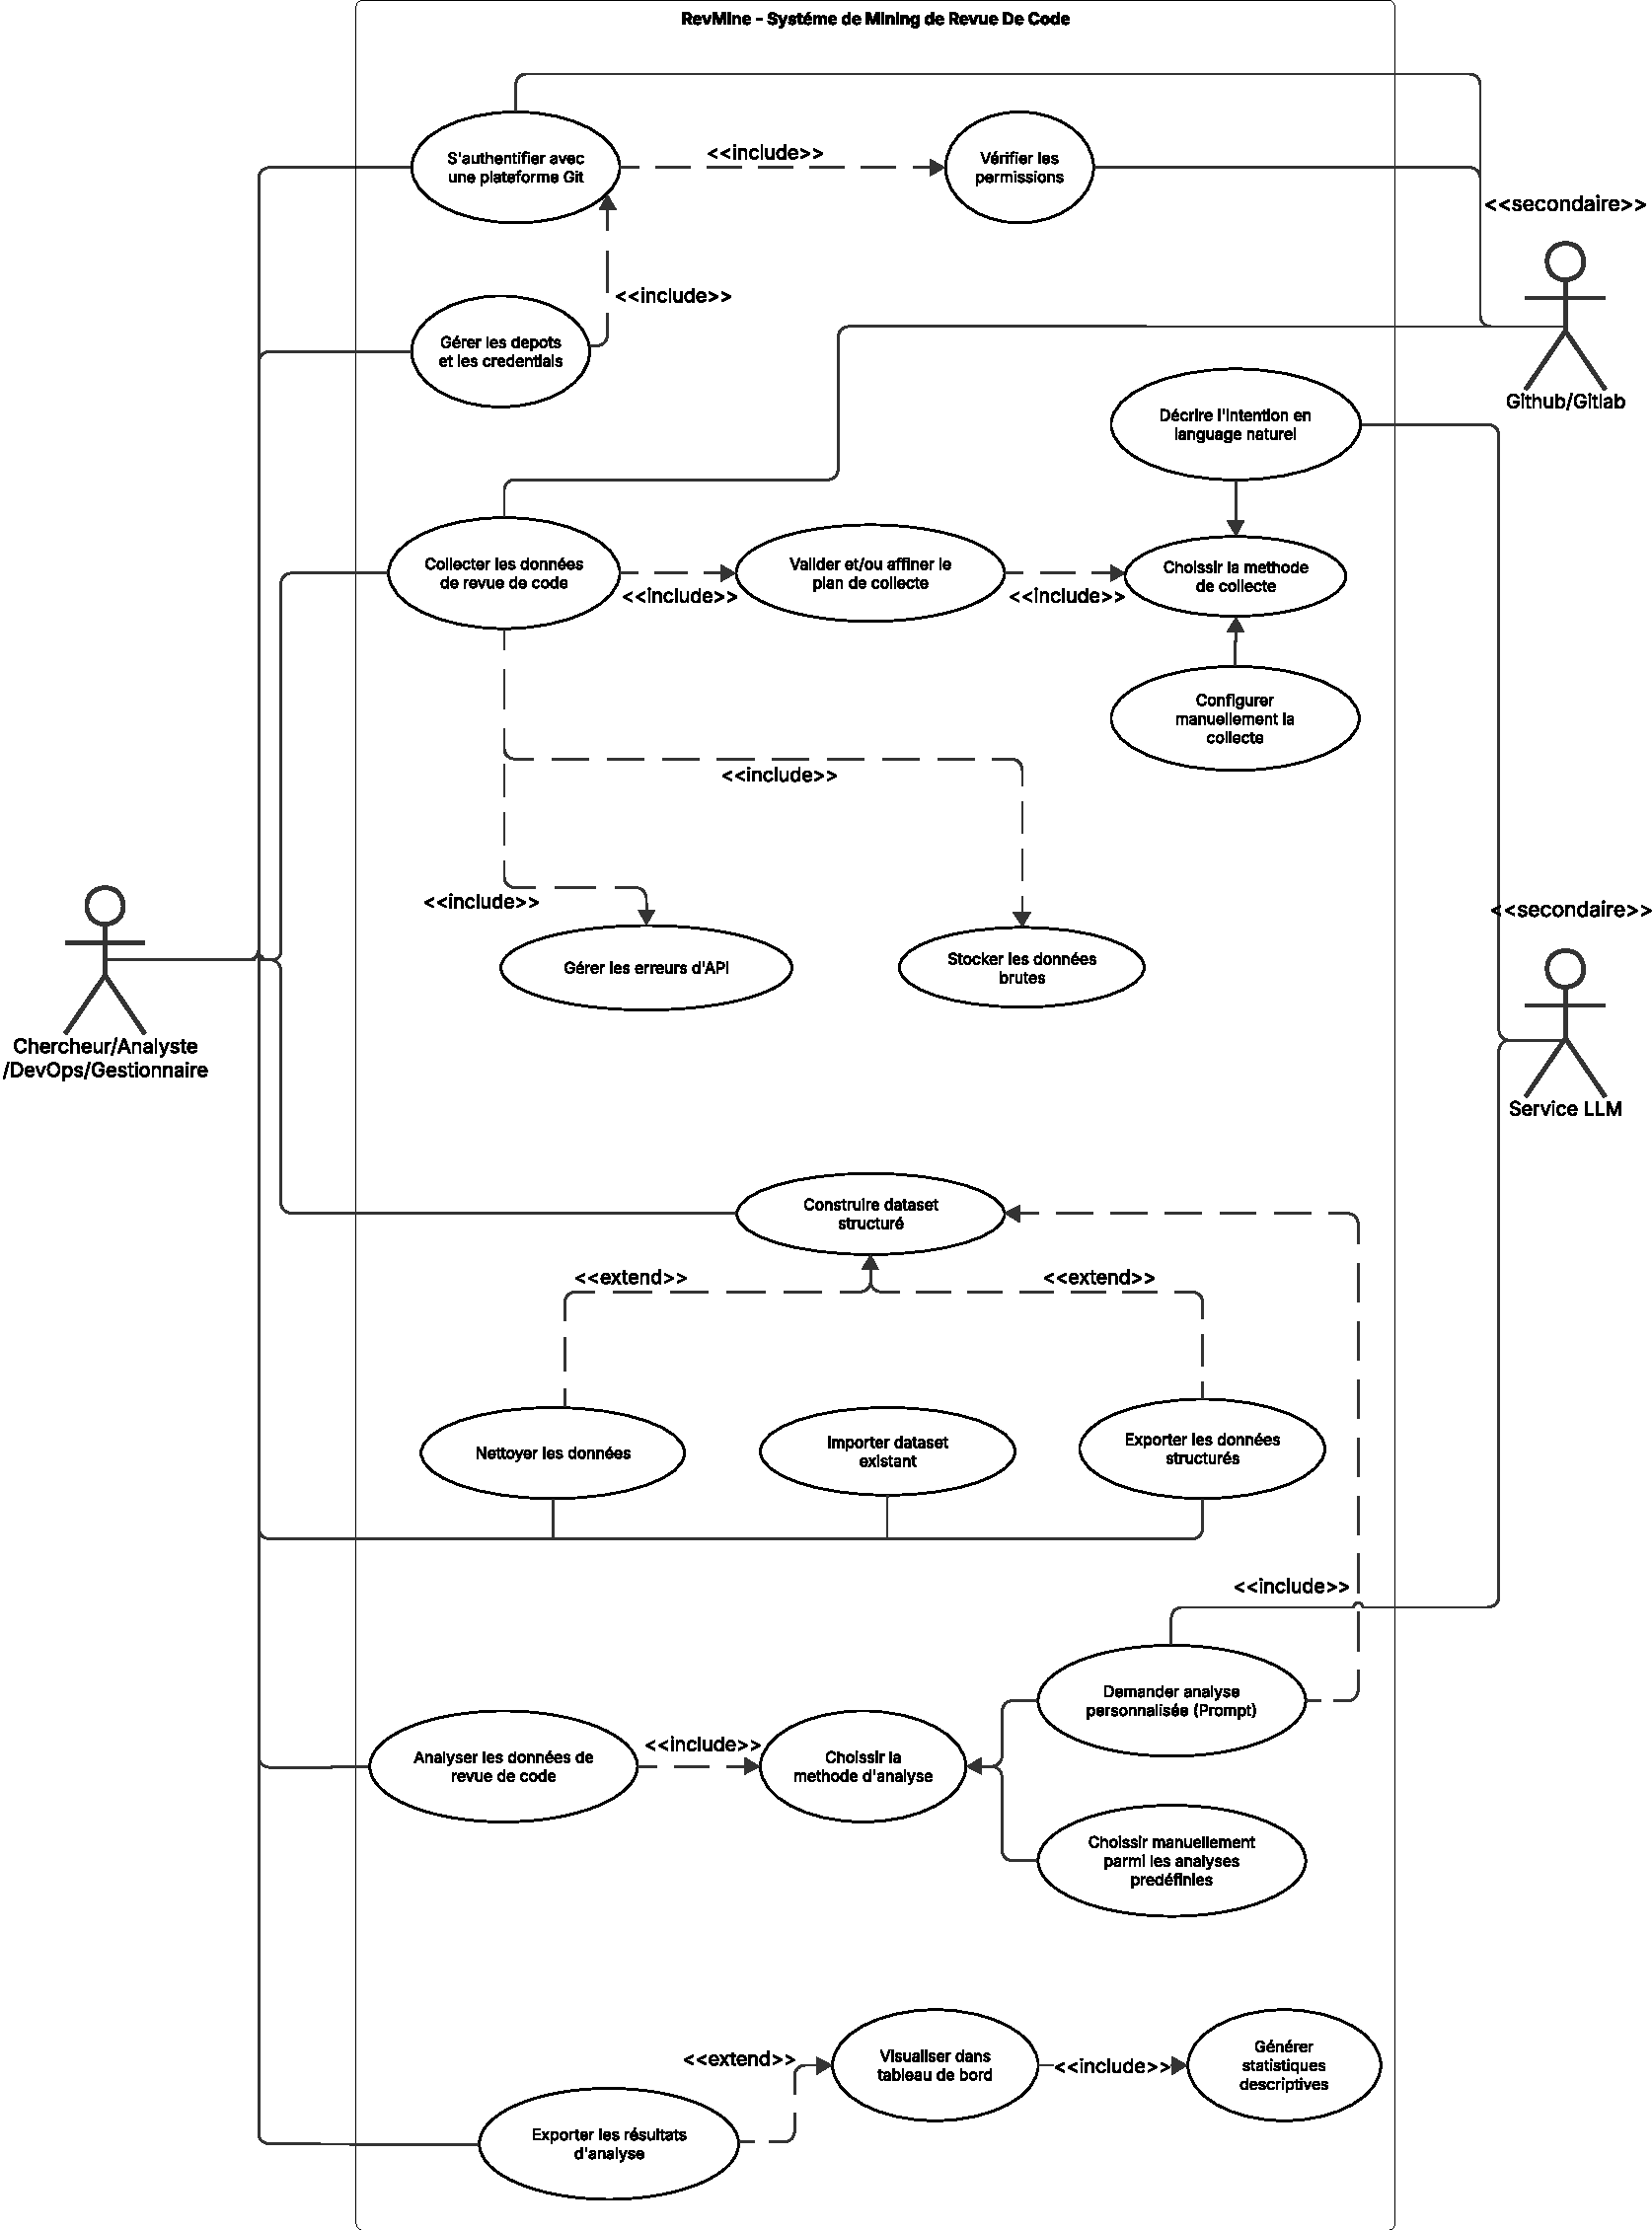
\includegraphics[width=\textwidth]{figures/useCaseDiagramm.pdf}
            \caption{Diagramme de cas d’utilisation}
            \label{fig:diagramme_cas_utilisation}
        \end{figure}

\subsection{Documentation des cas d'utillisation}
Parmi l’ensemble des cas d’utilisation identifiés, deux fonctionnalités principales se distinguent par leur rôle central dans le système RevMine : la collecte et l’analyse des données. Dans ce qui suit, nous présentons une description détaillée de ces cas d’utilisation, en précisant leurs acteurs, leurs préconditions ainsi que les différents scénarios d’exécution.


\subsubsection*{Cas d'utillisation de collecte des données de revue}
La collecte des données constitue une étape centrale du système RevMine. Après l’importation d’un dépôt depuis GitHub ou GitLab, l’utilisateur configure les paramètres de collecte en sélectionnant les endpoints et les filtres associés (branche, plage temporelle, état des PR/MR), ou en exprimant directement ses besoins en langage naturel afin de générer automatiquement un plan de collecte.

Ce plan est ensuite présenté à l’utilisateur, qui peut le valider ou l’ajuster avant son exécution. Une fois la collecte lancée, le système extrait les données via les API des plateformes et les sauvegarde sous un format structuré, en vue de leur exploitation dans les phases d’analyse.

\begin{tabularx}{\textwidth}{|l|X|}
\hline

\textbf{Nom du cas d’utilisation :} & Collecter les données de revue de code \\ \hline
\textbf{ID :} & UC1 \\ \hline

\textbf{Description :} & 
Ce cas d’utilisation décrit le processus permettant à un utilisateur de collecter les données de revue de code à partir d’un projet GitHub ou GitLab. \\ \hline

\textbf{Acteurs primaires :} & Chercheur / Analyste / DevOps / Gestionnaire \\ \hline
\textbf{Acteurs secondaires :} & API GitHub / GitLab \\ \hline

\textbf{Préconditions :} & 
\begin{itemize}
    \item L’utilisateur est authentifié sur la plateforme cible
    \item Le dépôt à analyser est importé dans l’espace de travail
\end{itemize} \\ \hline

\textbf{Enchaînement principal :} & 
\begin{enumerate}
    \item L’utilisateur sélectionne le dépôt à analyser
    \item Le système propose deux modes de collecte :
    \begin{itemize}
        \item Configuration manuelle
        \item Collecte via un prompt en langage naturel
    \end{itemize}

    \item \textbf{Cas 1 : Configuration manuelle}
    \begin{itemize}
        \item L’utilisateur sélectionne la branche cible (par défaut : \textit{main})
        \item L’utilisateur choisit les endpoints à interroger
        \item L’utilisateur définit la fenêtre temporelle (date de début et date de fin)
        \item L’utilisateur sélectionne le type de PR/MR (open, closed, merged)
        \item L’utilisateur lance la collecte
    \end{itemize}

    \item \textbf{Cas 2 : Collecte via prompt}
    \begin{itemize}
        \item L’utilisateur exprime ses besoins de collecte en langage naturel
        \item Le système génère automatiquement un plan de collecte
    \end{itemize}

    \item Le système affiche le plan de collecte généré
    \item L’utilisateur peut valider ou modifier les paramètres (branche, endpoints, filtres, etc.)
    \item Une fois validée, la collecte est lancée
    \item Le système extrait les données via les API et les sauvegarde sous forme structurée
\end{enumerate} \\ \hline

\textbf{Postconditions :} & 
\begin{itemize}
    \item Les données de revue de code sont collectées et stockées
    \item Des statistiques générales sur les données collectées peuvent être affichées
    \item L’utilisateur peut :
    \begin{itemize}
        \item Mettre en pause ou arrêter la collecte
        \item Télécharger les données brutes
    \end{itemize}
\end{itemize} \\ \hline

\textbf{Scénarios alternatifs :} & 
\begin{itemize}
    \item \textbf{Erreur lors de la collecte :}
    En cas d’erreur (réseau ou API), les données déjà collectées sont sauvegardées. Une notification informe l’utilisateur de l’arrêt du processus, avec possibilité de reprise ultérieure.

    \item \textbf{Modification du plan de collecte :}
    Si le plan généré ne correspond pas aux attentes, l’utilisateur peut le modifier avant validation.
\end{itemize} \\ \hline

\end{tabularx}



\subsubsection*{Cas d'utillisation d'analyse des données de revue de code}

L’analyse des données de revue de code permet d’exploiter les informations collectées afin d’en extraire des indicateurs pertinents. À partir de données préalablement collectées ou importées, et enrichies par le calcul de métriques (lead time, code churn, etc.), l’utilisateur peut explorer et affiner les données à l’aide de filtres tels que les auteurs, les types de fichiers, les plages temporelles ou des mots-clés.

L’analyse peut être réalisée soit à travers des options prédéfinies, soit en exprimant les besoins en langage naturel. Le système génère alors des visualisations interactives et personnalisables, facilitant l’interprétation des résultats et leur exploitation.

\begin{tabularx}{\textwidth}{|l|X|}
\hline

\textbf{Nom du cas d’utilisation :} & Analyser les données de revue de code \\ \hline
\textbf{ID :} & UC2 \\ \hline

\textbf{Description :} & 
Ce cas d’utilisation décrit le processus permettant à un utilisateur d’analyser les données de revue de code collectées. \\ \hline

\textbf{Acteurs primaires :} & Chercheur / Analyste / DevOps / Gestionnaire \\ \hline
\textbf{Acteurs secondaires :} & Service LLM \\ \hline

\textbf{Préconditions :} & 
\begin{itemize}
    \item Les données sont disponibles (collectées ou importées)
    \item Les métriques nécessaires sont calculées, ou un dataset contenant les métriques est fourni
\end{itemize} \\ \hline

\textbf{Enchaînement principal :} & 
\begin{enumerate}
    \item L’utilisateur sélectionne le dataset à analyser
    \item L’utilisateur peut nettoyer et filtrer les données (auteurs, types de fichiers, plage temporelle, mots-clés, etc.)
    \item L’utilisateur choisit le mode d’analyse :
    \begin{itemize}
        \item Analyse manuelle
        \item Analyse via prompt en langage naturel
    \end{itemize}

    \item \textbf{Cas 1 : Analyse manuelle}
    \begin{itemize}
        \item L’utilisateur sélectionne parmi les analyses prédéfinies (ex. : collaboration, performance des contributeurs, évolution des métriques, etc.)
        \item Le système génère des visualisations et des graphiques adaptés
        \item L’utilisateur explore les résultats à travers ces visualisations
        \item Les graphiques sont ajustables et personnalisables selon les besoins
    \end{itemize}

    \item \textbf{Cas 2 : Analyse via prompt}
    \begin{itemize}
        \item L’utilisateur exprime son besoin en langage naturel
        \item Le système génère automatiquement des visualisations correspondant à la demande
    \end{itemize}
\end{enumerate} \\ \hline

\textbf{Postconditions :} & 
\begin{itemize}
    \item Les résultats d’analyse sont affichés sous forme de tableaux de bord et de graphiques
    \item Des statistiques générales sont générées
    \item L’utilisateur peut exporter les résultats
    \item L’historique des analyses est accessible
\end{itemize} \\ \hline

\textbf{Scénarios alternatifs :} & 
\begin{itemize}
    \item \textbf{Métriques manquantes :}
    Si certaines analyses ne peuvent être réalisées en raison de l’absence de métriques, le système propose de les calculer à partir des données brutes disponibles.
\end{itemize} \\ \hline

\end{tabularx}

\newpage
\subsection{Diagrammes d'activité}
Afin de compléter la modélisation des cas d’utilisation, des diagrammes d’activité sont proposés pour illustrer le déroulement des principaux processus du système. Ces diagrammes permettent de représenter de manière dynamique les différentes étapes ainsi que les enchaînements des actions réalisées lors de l’exécution des fonctionnalités clés.

\subsubsection*{Configuration de Collecte des Données}
 \begin{figure}[H]
            \centering
            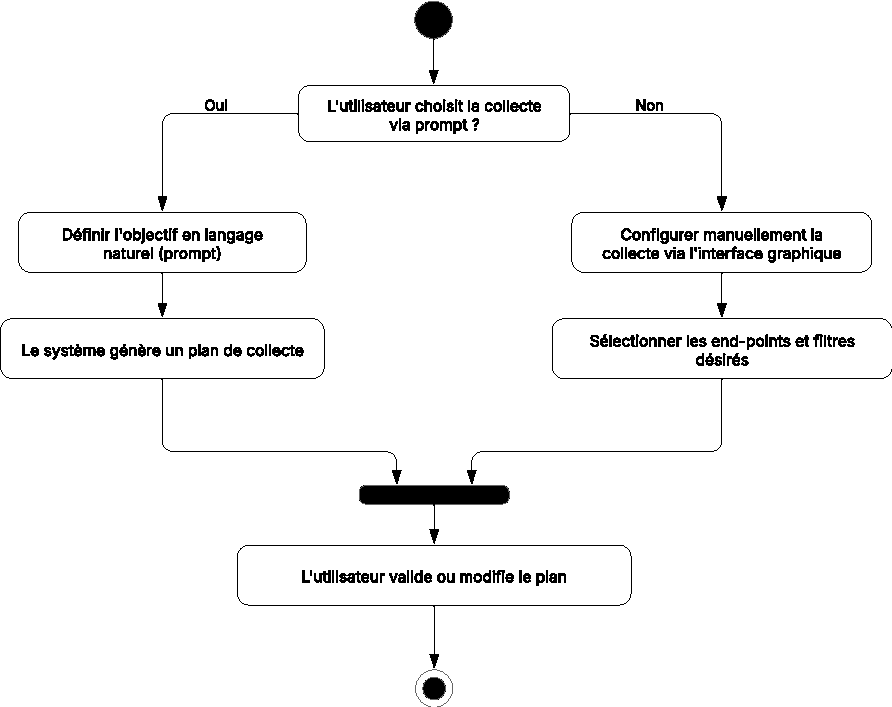
\includegraphics[width=\textwidth]{figures/Diagramme_activite2.pdf}
            \caption{Diagramme d’activité – Création et validation du plan de collecte.}
            \label{fig:activite_collecte_configuration}
        \end{figure}

\subsubsection*{Post-Collecte des Données}
\begin{figure}[H]
    \centering
    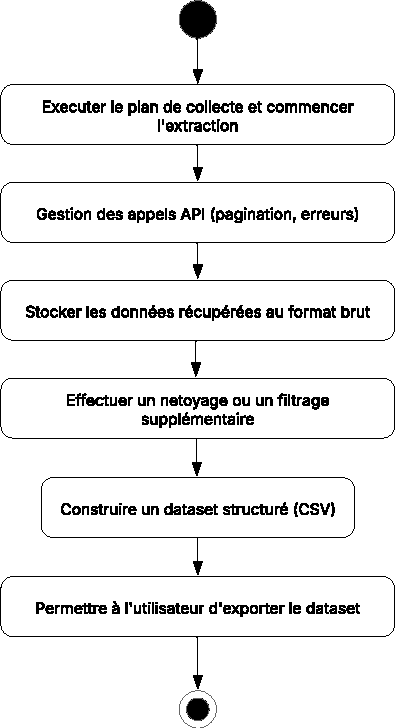
\includegraphics[height=18cm, keepaspectratio]{figures/Diagramme_activite1.pdf}
    \caption{Diagramme d’activité – Filtrage et Nettoyage des données collectées.}
    \label{fig:activite_post_collecte}
\end{figure}

\subsubsection*{L'Analyse des Données}
 \begin{figure}[H]
            \centering
            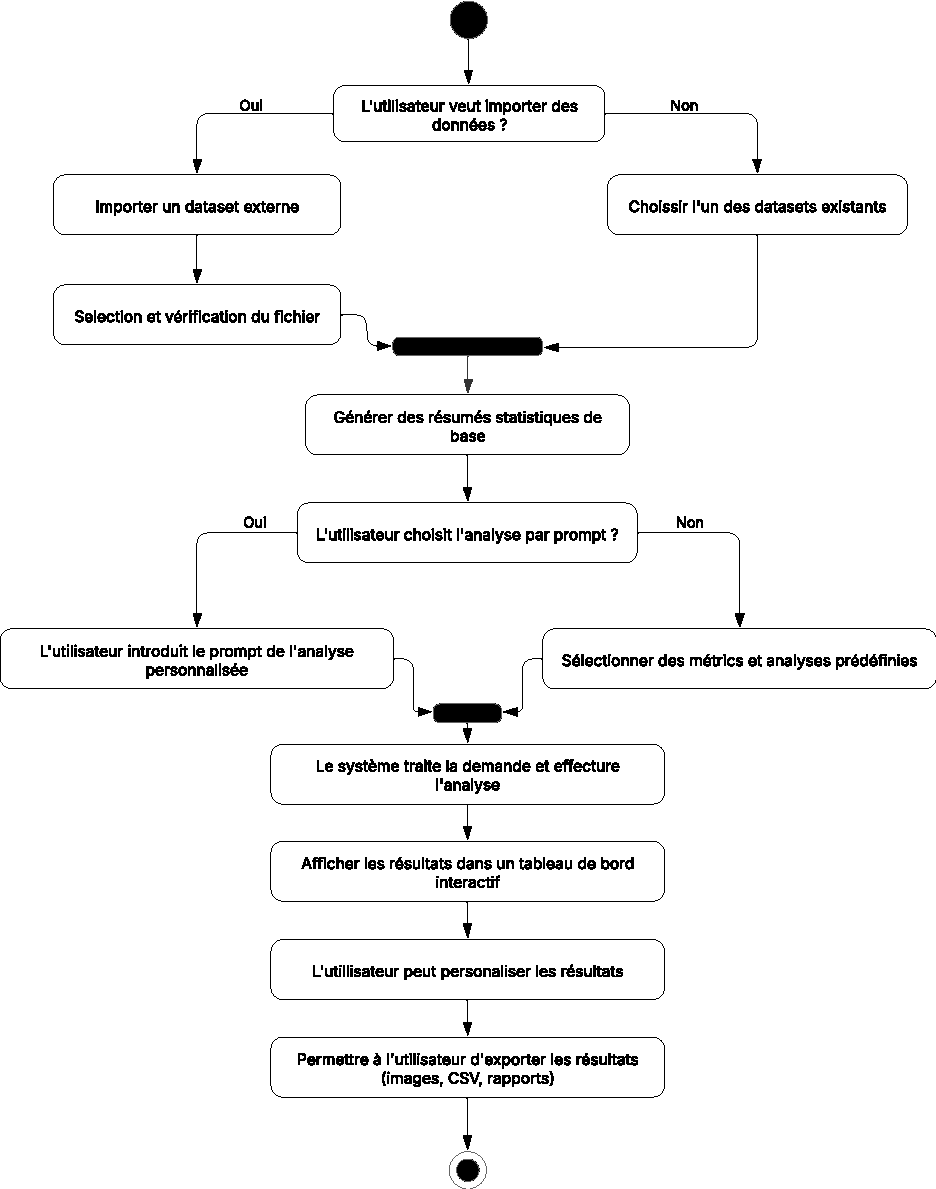
\includegraphics[width=\textwidth]{figures/Diagramme_activite3.pdf}
            \caption{Diagramme d’activité – Configuration, exécution et visualisation des analyses.}
            \label{fig:activite_analyse_donnees}
        \end{figure}




\section{Traçabilité des besoins}
Afin d’assurer la cohérence entre les besoins fonctionnels identifiés et la modélisation du système, une matrice de traçabilité est établie. Elle permet de vérifier que chaque cas d’utilisation couvre bien un ou plusieurs besoins fonctionnels.

\begin{tabularx}{\textwidth}{|l|X|}
\hline

\textbf{Cas d’utilisation} & \textbf{Besoins fonctionnels couverts} \\ \hline

S’authentifier avec une plateforme Git & BF2, BF3, BF4 \\ \hline
Vérifier les permissions & BF4 \\ \hline
Gérer les dépôts et les credentials & BF1, BF2, BF3, BF5 \\ \hline
Collecter les données de revue de code & BF5, BF6, BF7, BF8, BF9, BF10, BF11 \\ \hline
Choisir la méthode de collecte & BF6, BF7 \\ \hline
Configurer manuellement la collecte & BF6 \\ \hline
Décrire l’intention en langage naturel & BF7 \\ \hline
Valider et/ou affiner le plan de collecte & BF8 \\ \hline
Gérer les erreurs d’API & BF10 \\ \hline
Stocker les données brutes & BF11 \\ \hline
Construire dataset structuré & BF11, BF12, BF13, BF14, BF20 \\ \hline
Nettoyer les données & BF12 \\ \hline
Importer dataset existant & BF13 \\ \hline
Exporter les données structurées & BF20 \\ \hline
Analyser les données de revue de code & BF14, BF15, BF16, BF17, BF18, BF19, BF20 \\ \hline
Choisir la méthode d’analyse & BF15, BF16 \\ \hline
Demander analyse personnalisée (Prompt) & BF15 \\ \hline
Choisir manuellement parmi les analyses prédéfinies & BF16 \\ \hline
Visualiser dans tableau de bord & BF17, BF18, BF19 \\ \hline
Générer statistiques descriptives & BF18 \\ \hline
Exporter les résultats d’analyse & BF20 \\ \hline

\end{tabularx}




\section{Conclusion}
Ce chapitre a permis d’établir les fondements analytiques de la solution RevMine à travers une étude structurée des besoins. Nous avons tout d’abord présenté la méthodologie suivie, puis identifié les différents acteurs du système avant de définir les besoins fonctionnels et non fonctionnels.

Ces besoins ont ensuite été validés afin d’assurer leur cohérence et leur adéquation avec les objectifs du projet, aussi bien du point de vue académique qu’industriel. Par la suite, ils ont été modélisés à travers un diagramme de cas d’utilisation, une documentation des cas principaux, des diagrammes d’activité ainsi qu’une matrice de traçabilité permettant de vérifier leur couverture.

Cette analyse constitue ainsi un socle solide pour la suite du développement. Dans le chapitre suivant, nous aborderons la phase de conception, où les besoins identifiés seront traduits en une architecture détaillée et en choix de conception permettant de structurer la solution proposée.
